
% === Auto-generated by make_latex_compare_flat.py ===
% Requires in preamble: \usepackage{graphicx,subcaption}
% Tip: compile with: latexmk -pdf

\begin{figure*}[htbp]\centering
\begin{subfigure}[htbp]{0.8\textwidth}
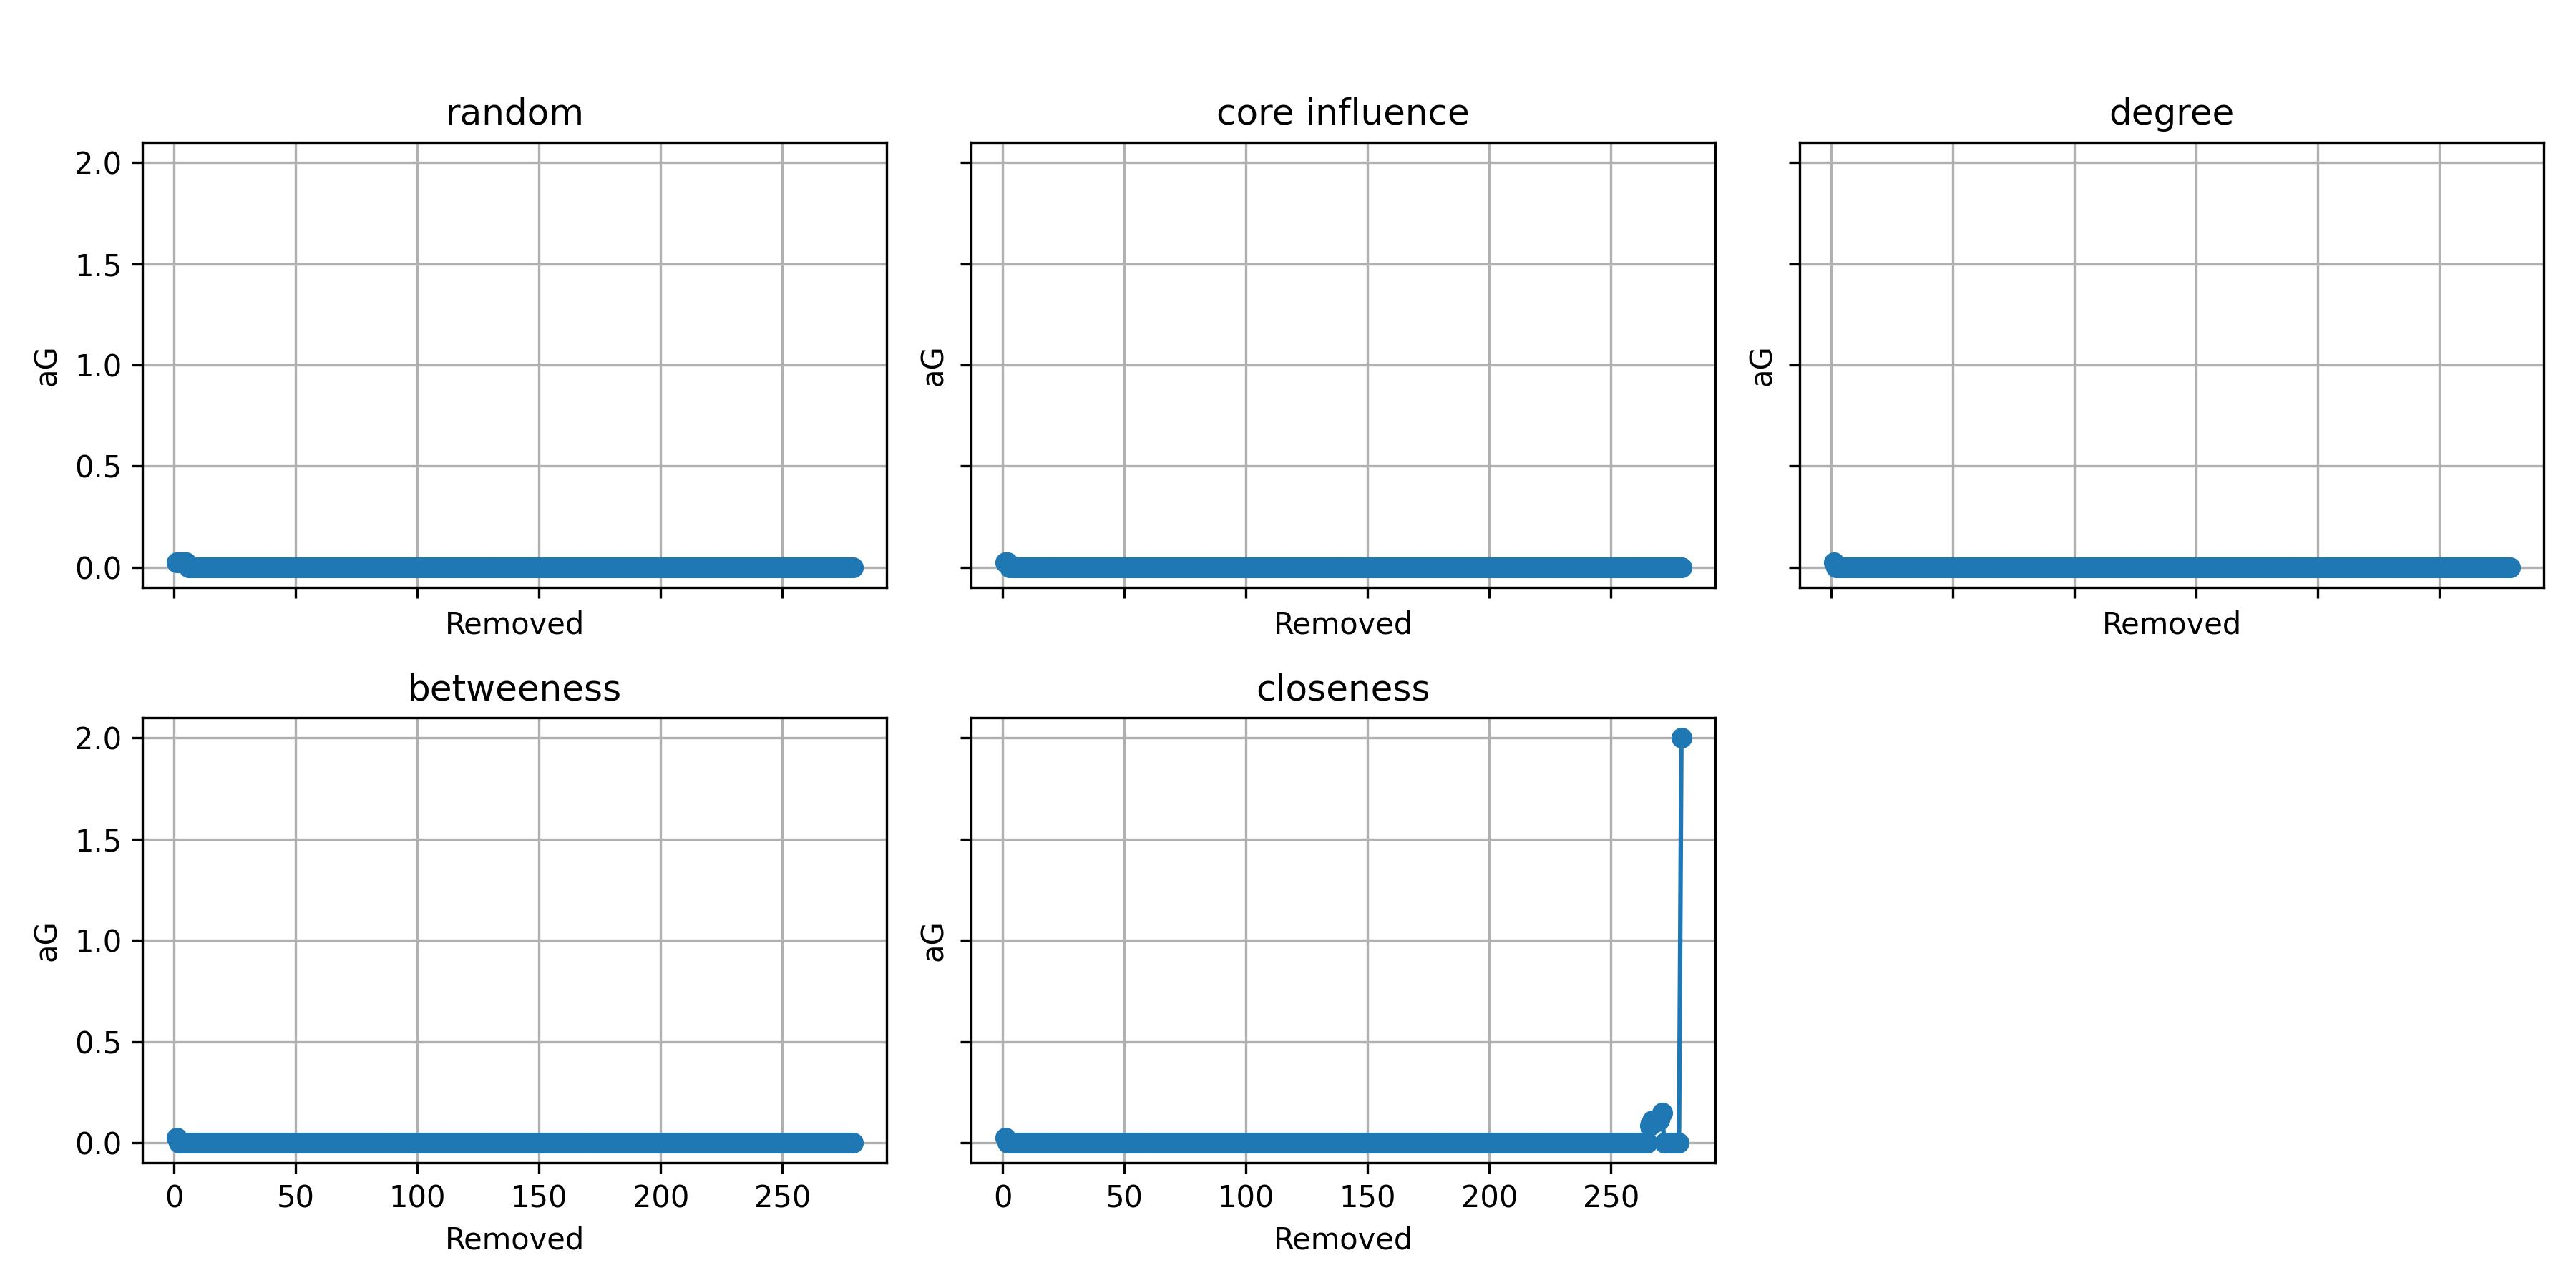
\includegraphics[width=\linewidth]{images/isis-links.json_compare_aG.jpg}
\caption{isis-links: $a(G)$}
\label{fig:aG_isis-links_compare}
\end{subfigure}
\hfill
\caption{{{caption}}}\label{{{label}}}\end{figure*}

\begin{figure*}[htbp]\centering
\begin{subfigure}[htbp]{0.8\textwidth}
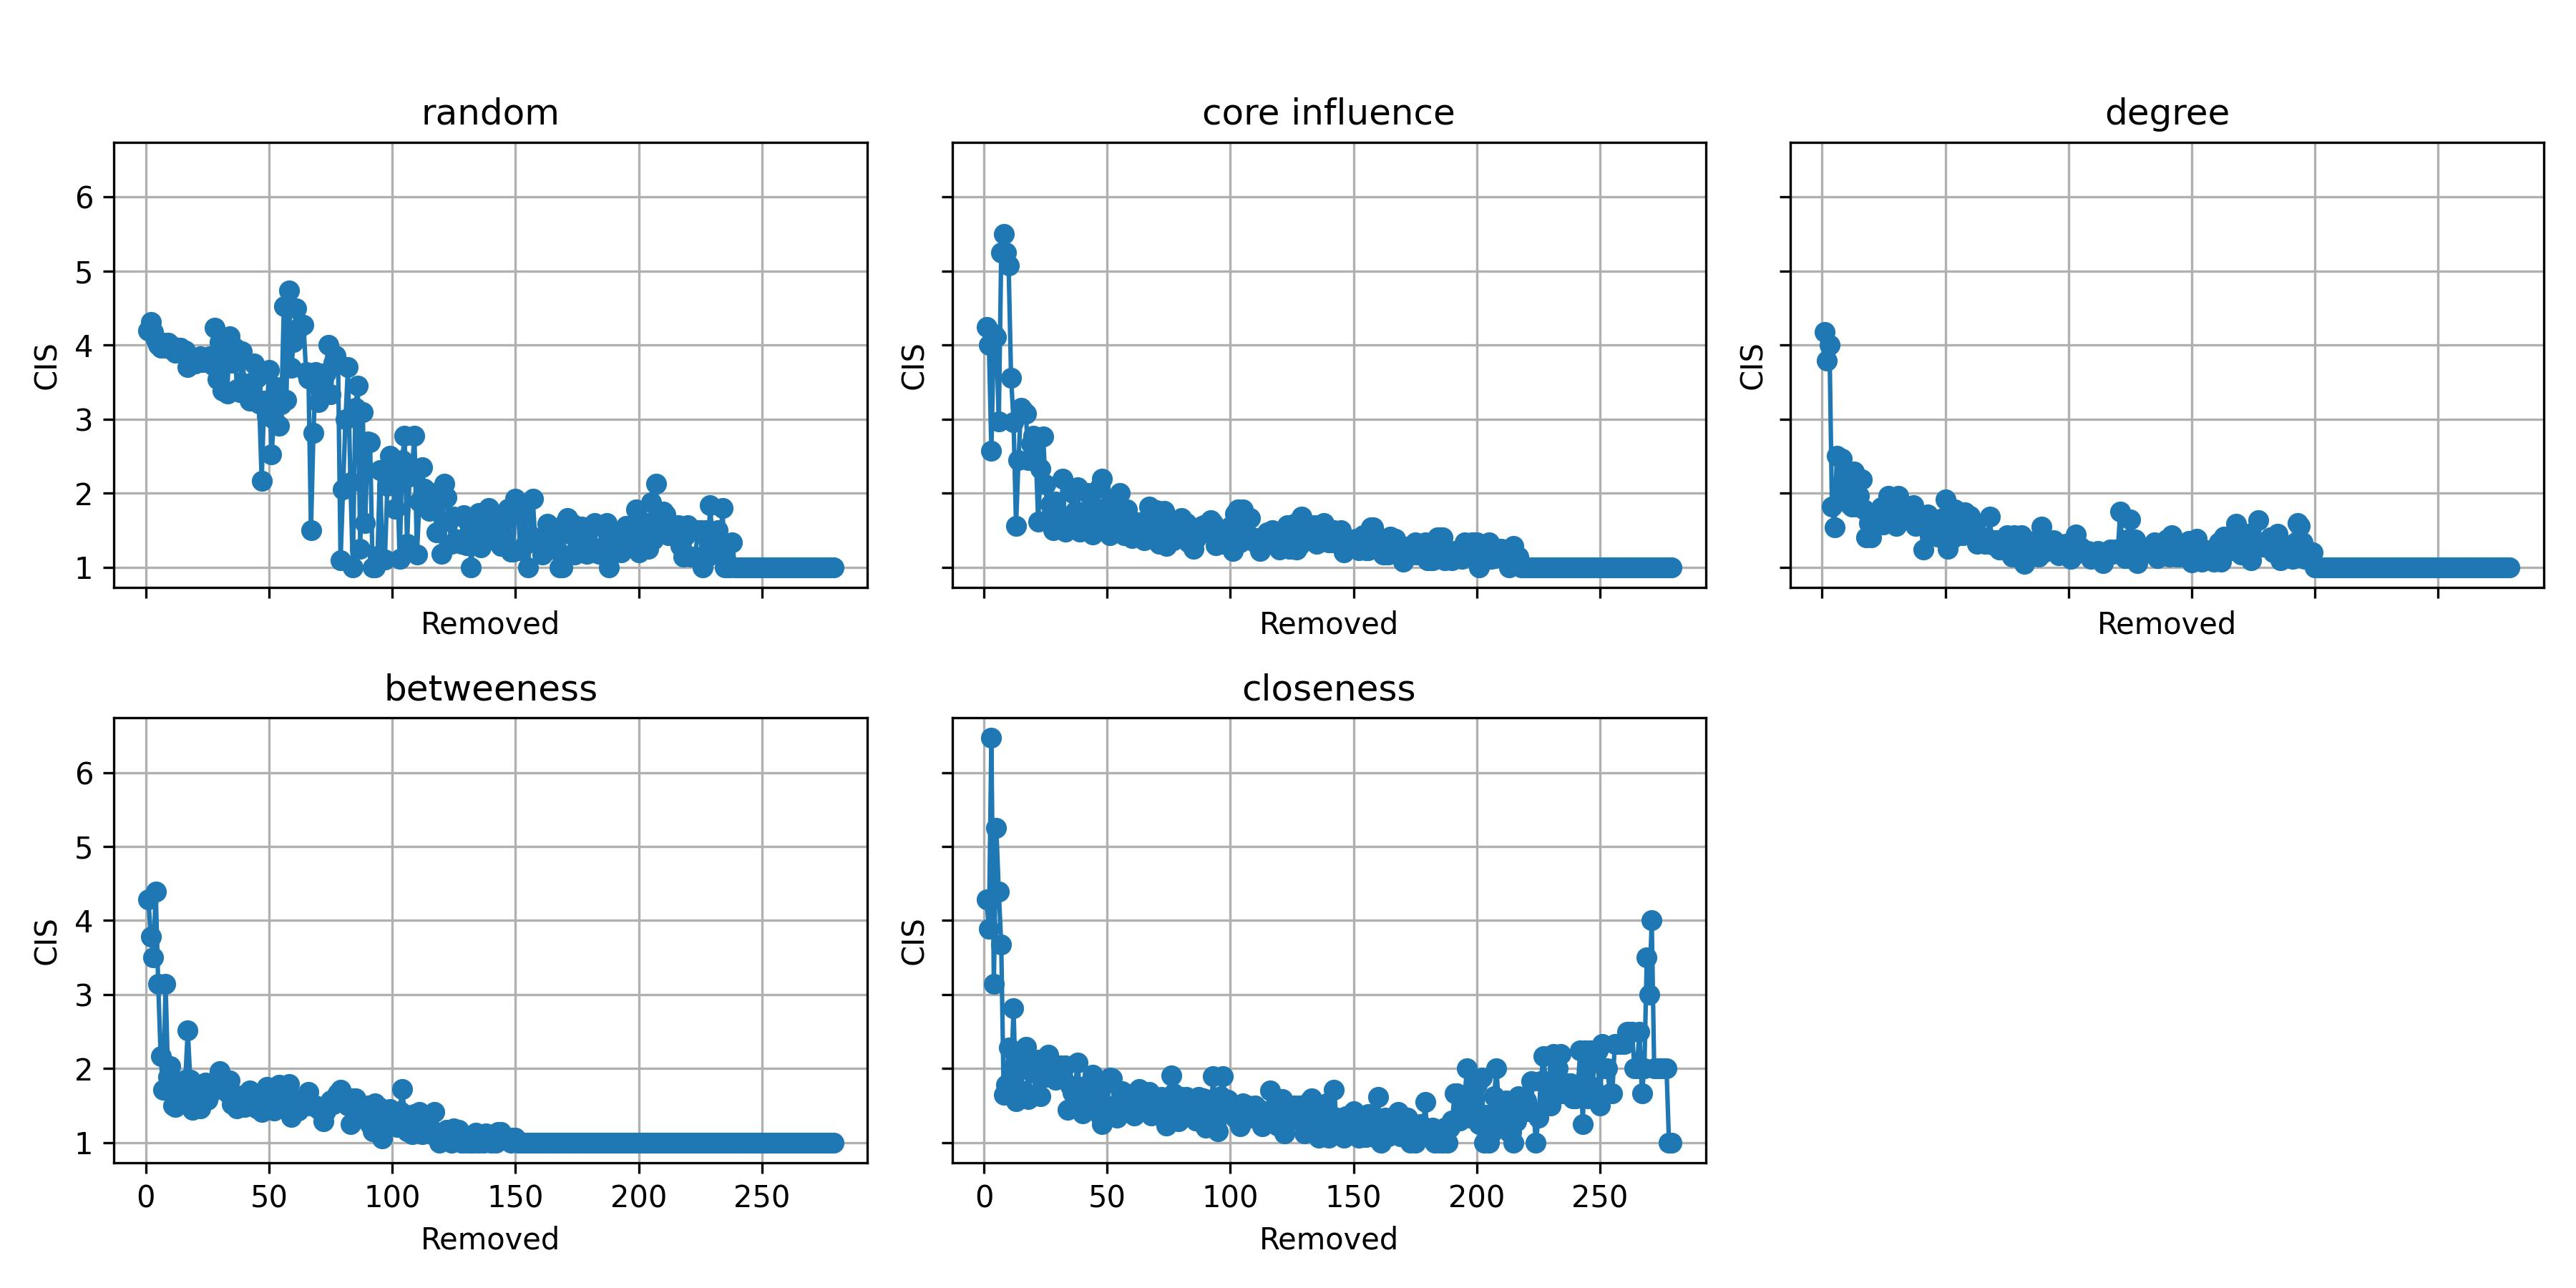
\includegraphics[width=\linewidth]{images/isis-links.json_compare_CIS.jpg}
\caption{isis-links: CIS}
\label{fig:CIS_isis-links_compare}
\end{subfigure}
\hfill
\caption{{{caption}}}\label{{{label}}}\end{figure*}

\begin{figure*}[htbp]\centering
\begin{subfigure}[htbp]{0.8\textwidth}
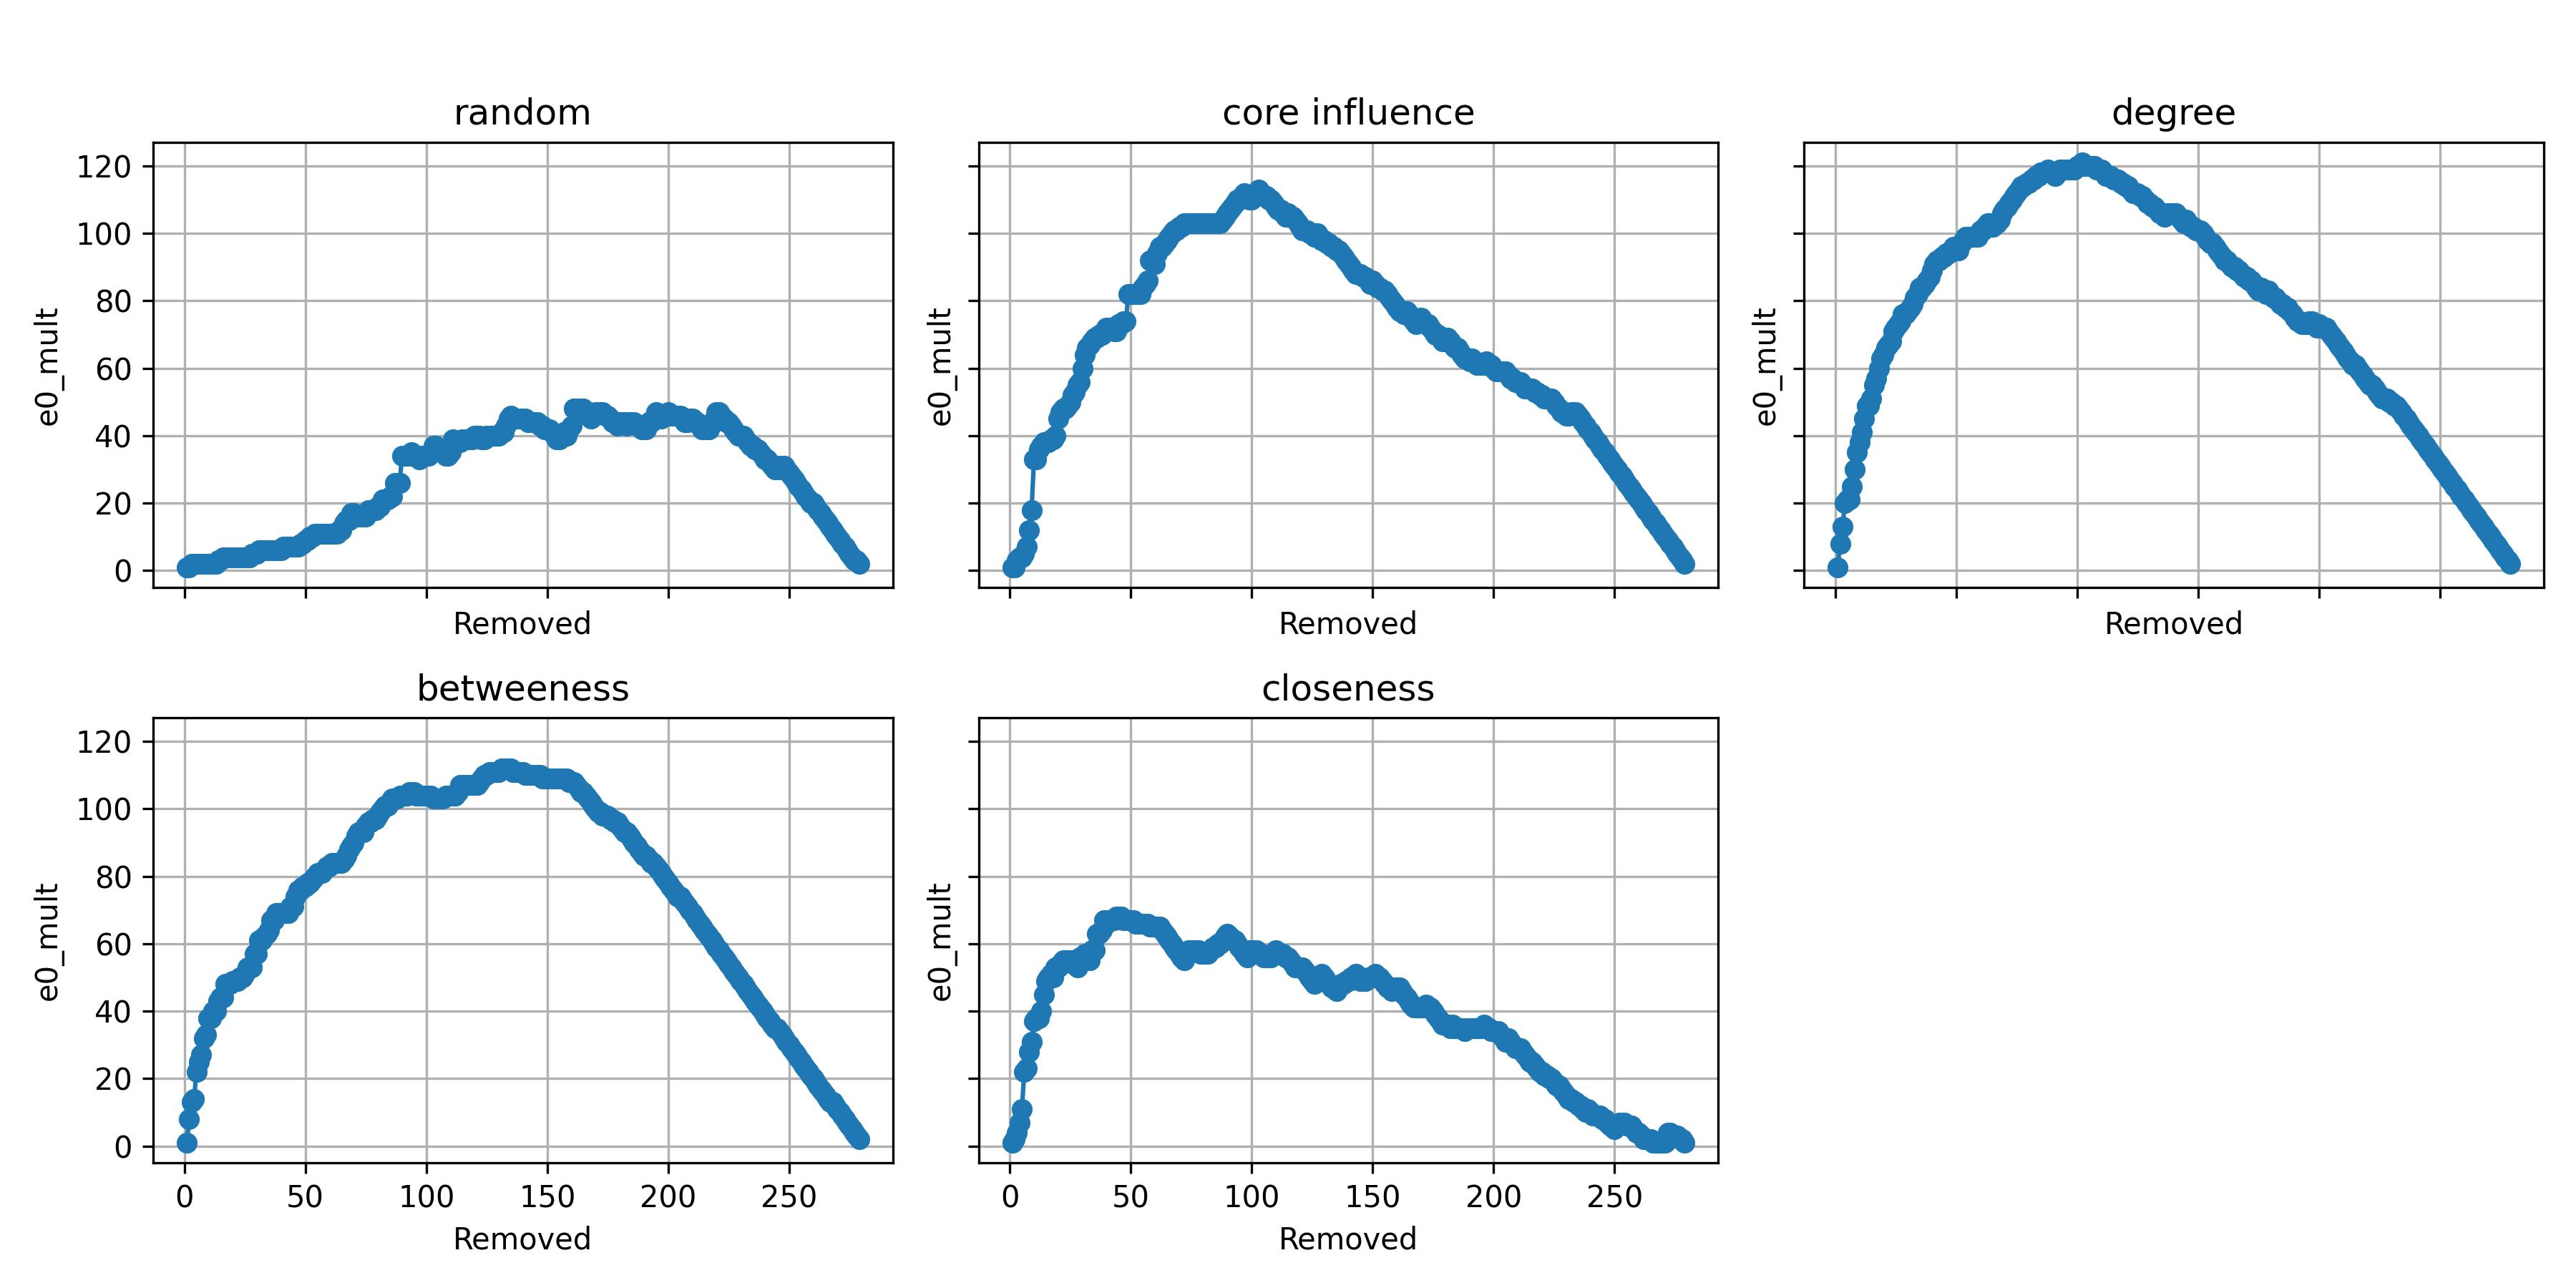
\includegraphics[width=\linewidth]{images/isis-links.json_compare_e0_mult.jpg}
\caption{isis-links: $e0$}
\label{fig:e0_mult_isis-links_compare}
\end{subfigure}
\hfill
\caption{{{caption}}}\label{{{label}}}\end{figure*}

\begin{figure*}[htbp]\centering
\begin{subfigure}[htbp]{0.8\textwidth}
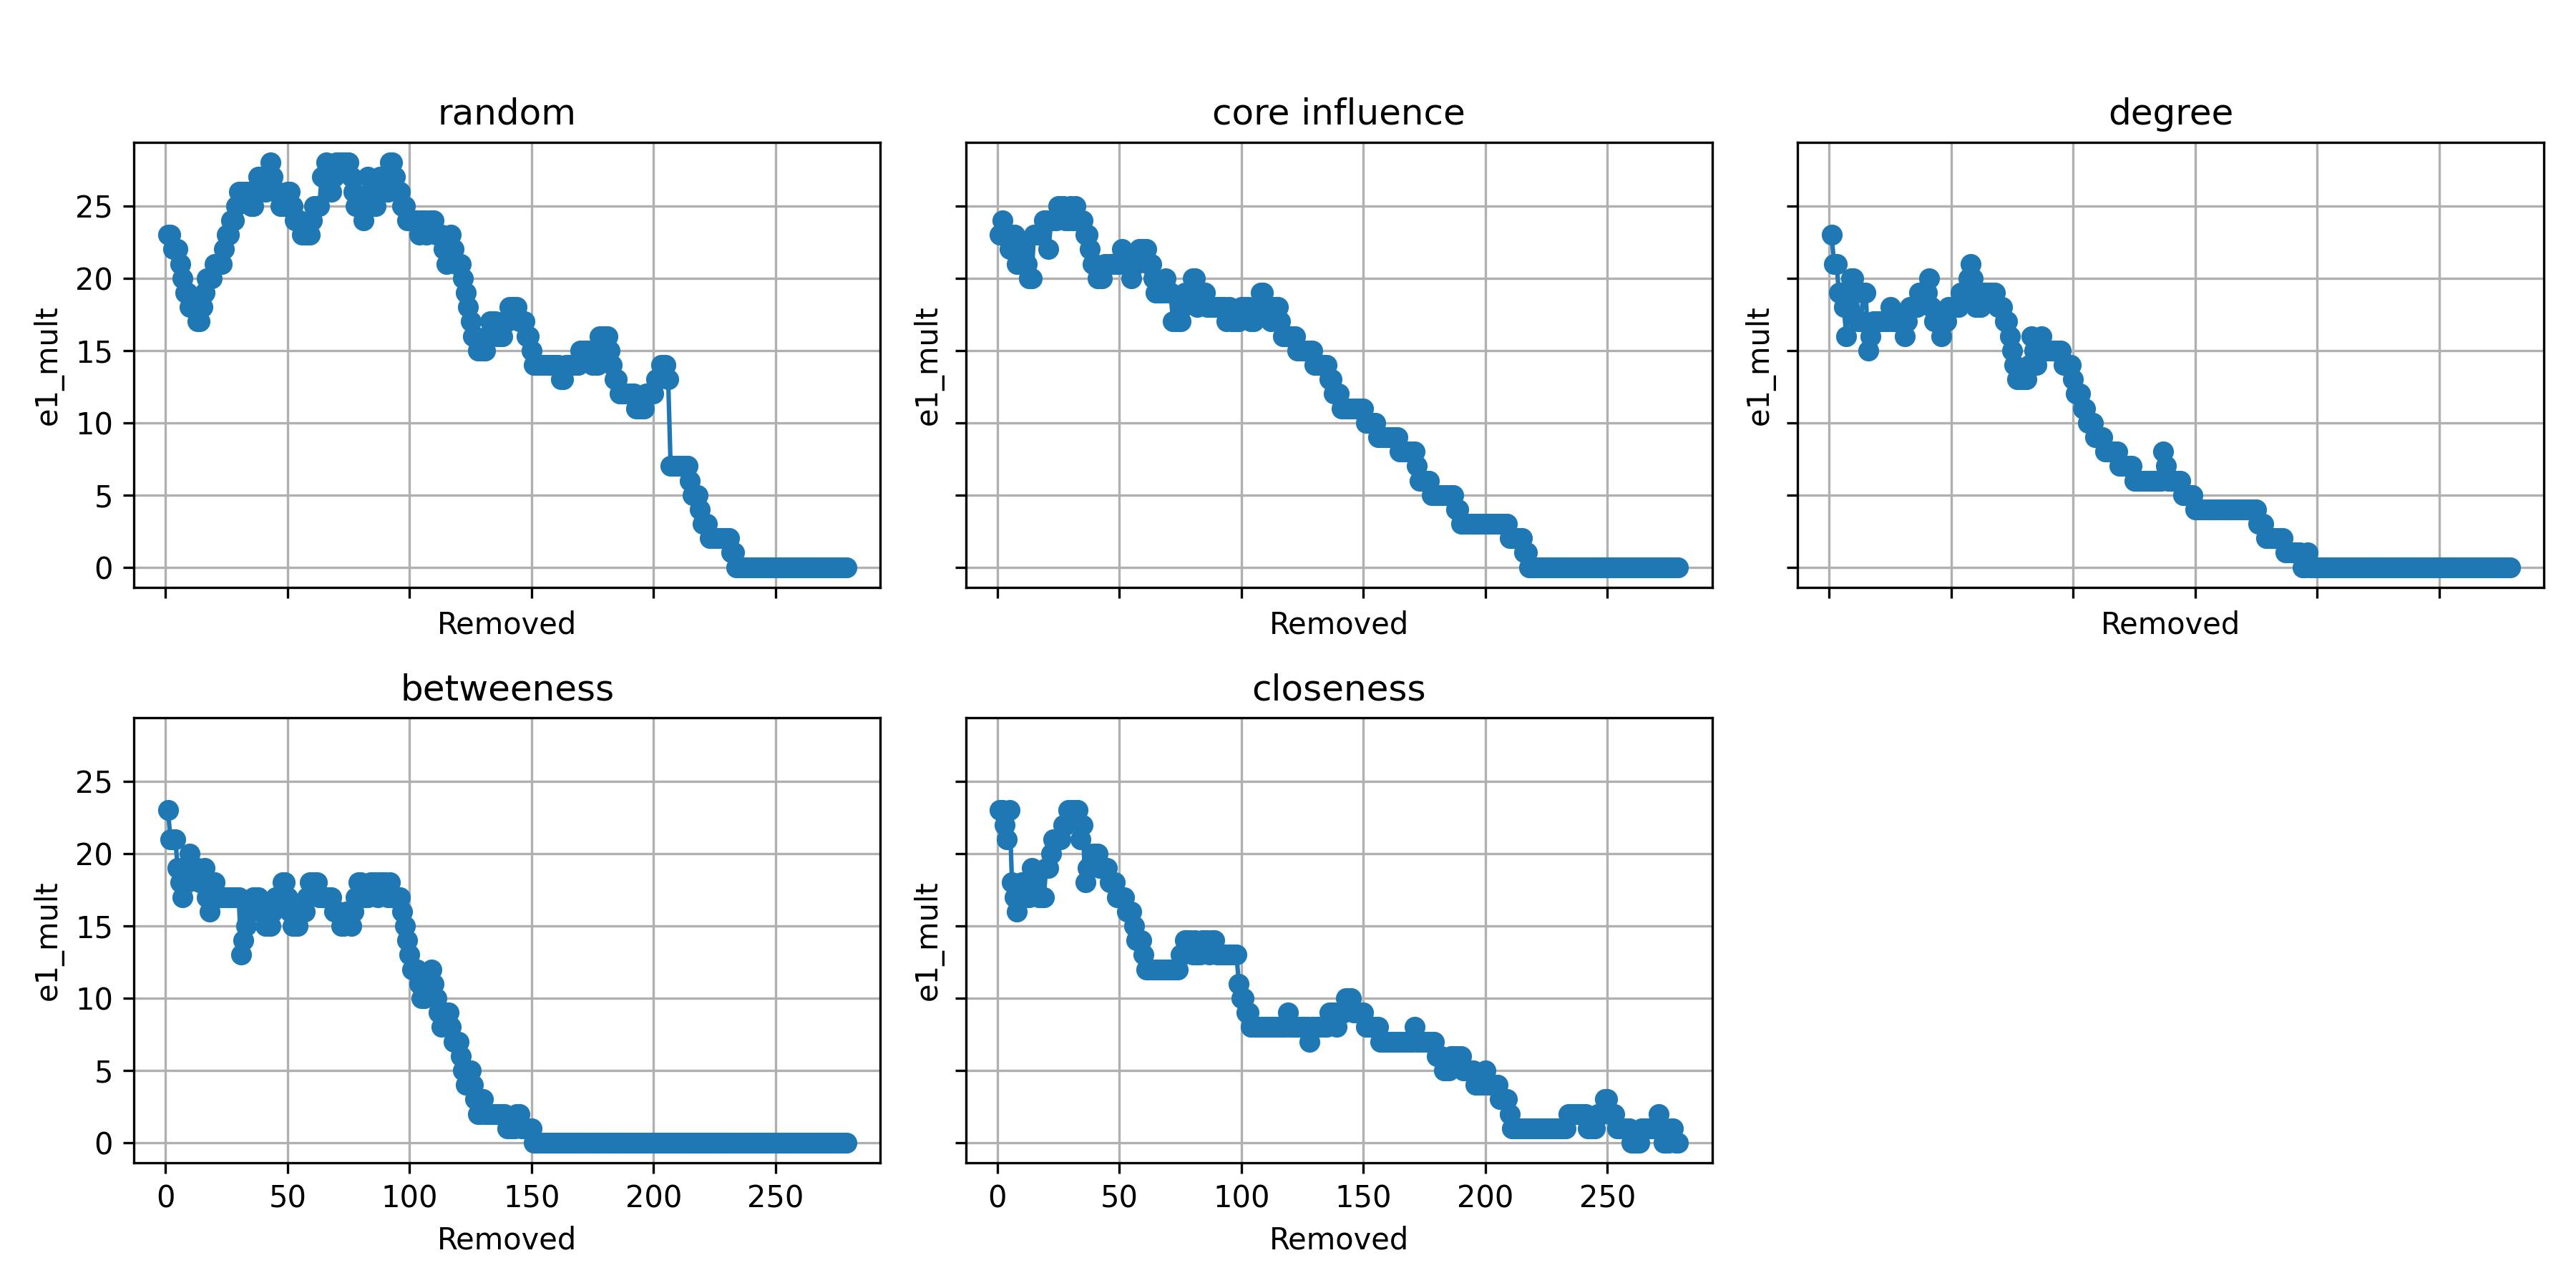
\includegraphics[width=\linewidth]{images/isis-links.json_compare_e1_mult.jpg}
\caption{isis-links: $e1$}
\label{fig:e1_mult_isis-links_compare}
\end{subfigure}
\hfill
\caption{{{caption}}}\label{{{label}}}\end{figure*}
